\subsection{Analiza systemów informatycznych z użyciem sieci Petriego}

\textbf{Sieci Petriego} – jest to matematyczna reprezentacja systemów rozproszonych. Umożliwiają one badanie zjawisk współbieżnych zachodzących w systemach wzajemnie się warunkujących w czasie. Uogólniają one teorię automatów. Podstawowa wersja sieci Petriego składa się z:


\begin{itemize}
	\item \textbf{miejsc} (odpowiadających warunkom),
	\item \textbf{przejść} (odpowiadających zdarzeniom),
	\item \textbf{łuków} (krawędzi, odpowiadających związkom między zdarzeniami i warunkami.
\end{itemize}

Aby opisać konkretny stan układu, potrzebne są żetony które można przemieszczać pomiędzy miejscami poprzez przejścia po krawędziach grafu. Oznaczeniami są:


\begin{itemize}
	\item \textbf{kropki} – żetony
	\item \textbf{prostokąty}(grube kreski) – przejścia
	\item \textbf{okręgi} – miejsca
	\item \textbf{strzałki} – krawędzie, łuki

\end{itemize}

Działanie sieci polega na przesuwaniu się znaczników między miejscami sieci.

\subsubsection{Własności sieci Petriego}

\begin{itemize}
	\item \textbf{Osiągalność} – sprawdzanie, czy dany stan jest osiągalny ze stanu początkowego (tzn. czy istnieje skończona liczba przejść, która prowadzi od znakowania początkowego do znakowania badanego).
	\item \textbf{Ograniczoność} – liczba znaczników w danym miejscu jest ograniczona.
	\item \textbf{Zachowawczość} – sieć Petriego jest zachowawcza, jeżeli liczba występujących w niej znaczników jest stała.
	\item \textbf{Żywotność} – określa liczbę możliwych wykonań przejścia. Sieć jest żywa, jeżeli z każdego oznakowania można osiągnąć inne oznakowania.
	\item \textbf{Odwracalność} – sieć jest odwracalna, jeżeli stan początkowy sieci jest osiągalny z każdego oznakowania.
\end{itemize}

Trzy główne metody analizy sieci Petriego:

\begin{itemize}
	\item \textbf{Grafy osiągalności} – opiera się ona na budowie drzewa osiągalności. Ze stanu początkowego odpala się wszystkie możliwe przejścia , które prowadzą do osiągalnych znakowań tworzących węzły grafu, z nich tworzone są kolejne, itd. W drzewie osiągalności można w sposób jednoznaczny dojść od korzenia do dowolnego innego węzła. Drzewo może być nieskończone.
	\item \textbf{Grafy pokrycia} - otrzymywany jest z drzewa pokrycia poprzez scalenie duplikujących się wierzchołków. Na podstawie skończonego grafu pokrycia możliwe jest badanie sieci o nieskończonym zbiorze znakowań.
	\item \textbf{Metody algebraiczne} (macierz incydencji). Definiuje się macierz wejść wyjść. W macierzy incydencji liczba wierszy to liczba miejsc, liczba kolumn to liczba przejść.
\end{itemize}

\subsubsection{Przykład sieci Petriego}

Chcemy zaprojektować oprogramowanie dla systemu kontroli sygnalizacji świetlnej. Zakładamy, że dane są dwa autonomiczne systemy sterujące sygnalizacją świetlną – jeden dla pojazdów i drugi dla ludzi. Należy je zsynchronizować.

\begin{figure}[H]
	\centering
	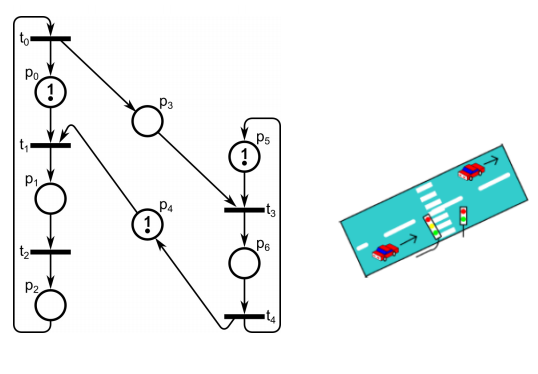
\includegraphics[width=0.7\linewidth]{K7.png}
	\caption{Przykładowa sieć}
\end{figure}


Znaczenie miejsc na rysunku 1.3 jest następujące:

\begin{itemize}
	\item p0, p1, p2 – światła uliczne dla aut, odpowiednio p0 – czerwone, p1 – żółte, p2 – zielone,
	\item p3, p4 – światła uliczne dla pieszych, odpowiednio p3 – czerwone, p4 – zielone,
	\item p5, p6 – miejsca służące do synchronizacji (np. flagi umieszczone w oprogramowaniu).
\end{itemize}

